\documentclass[12pt]{article}

\usepackage{afterpage}
\usepackage{amsmath}
\usepackage{changepage}
\usepackage{enumitem}
\usepackage{etoolbox}
\usepackage{fontspec}
\usepackage[letterpaper,margin=72pt]{geometry}
\usepackage{hyperref}
\usepackage{listings}
\usepackage{tikz}
\usepackage{titling}
\usepackage{xcolor}

\newbool{solutions}
\booltrue{solutions}
% \boolfalse{solutions}

\usetikzlibrary{calc}

\setsansfont{Inter}[Scale=MatchLowercase]
\setmonofont{Hack}[Scale=MatchLowercase]

\renewcommand{\familydefault}{\sfdefault}

\newenvironment{answer}{\begin{adjustwidth}{1cm}{}\itshape}{\end{adjustwidth}}

\lstset{
  basicstyle=\ttfamily,
}

\definecolor{uclablue}{RGB}{39,116,174}
\definecolor{uclagold}{RGB}{255,179,0}

\definecolor{solarizedred}{RGB}{220, 50, 47}
\definecolor{solarizedblue}{RGB}{38, 139, 210}
\definecolor{solarizedgreen}{RGB}{133, 153, 0}
\definecolor{solarizedpurple}{RGB}{108, 113, 196}

\colorlet{primarycolor}{uclablue}
\colorlet{secondarycolor}{uclagold}


\hypersetup{
  colorlinks=true,
  urlcolor=uclablue,
}

\setlist{nosep}

\parindent=0pt

\title{Midterm Exam Fall '21}
\author{Jon Eyolfson}
\date{October 26, 2021}

\begin{document}

\pagenumbering{gobble}

\begin{tikzpicture}[remember picture,overlay,shift={(current page.south west)}]
  \node (title) at (\paperwidth / 2, \paperheight * 2 / 3)
        {\huge \bfseries \thetitle};
  \node [anchor=south] at (title.north)
        {CS 111: Operating System Principles};
  \node [anchor=north] (author) at (title.south) {Instructor: \theauthor};

  \node (duration) at (\paperwidth / 2, \paperheight / 2)
        {Duration: 1 hour 50 minutes};
  \node [anchor=south] (date) at (duration.north) {\thedate};

  \draw (2 * \paperwidth / 3, \paperheight / 3)
        -- (\paperwidth / 3, \paperheight / 3);
  \node [anchor=north] at (\paperwidth / 2, \paperheight / 3) {Name};

  \draw (2 * \paperwidth / 3, \paperheight / 4)
        -- (\paperwidth / 3, \paperheight / 4);
  \node [anchor=north] at (\paperwidth / 2, \paperheight / 4) {Student ID};

  \node [align=center, anchor=north] at (\paperwidth / 2, \paperheight / 5)
        {This is a closed book exam.
        You are only permitted a pencil or pen. \\
        Answer the questions directly on the exam. \\
        \\
        If in doubt, write your assumptions and answer the question as best you
        can. \\
        There are 8 numbered pages (page 8 is blank if you need extra room). \\
        The pace of the midterm is approximately one point a minute. \\
        There are 100 total points. \\
        \\
        Good luck!};
\end{tikzpicture}

\newpage

\pagenumbering{arabic}

\textbf{(5 points)}
Explain the concept of virtualization and how it applies to operating systems.

\vspace{1em}

\ifbool{solutions}{
  \begin{answer}
    The concept of virtualization is making something believe it has exclusive
    access to a resource, when it's actually being shared. For instance virtual
    memory allows multiple processes to think they can access the entire memory
    while they actually share physical memory.
  \end{answer}
  \vspace{4em}
}{
  \vspace{8em}
}

\vspace{1em}

\textbf{(5 points)}
What service would you find in a monolithic kernel, but not in a microkernel?

\vspace{1em}

\ifbool{solutions}{
  \begin{answer}
    File systems / Device drivers / Advanced IPC
  \end{answer}
  \vspace{4em}
}{
  \vspace{8em}
}

\vspace{1em}

\textbf{(5 points)}
What should you use to monitor all system calls a process makes?

\vspace{1em}

\ifbool{solutions}{
  \begin{answer}
    You can use \texttt{strace} to monitor system calls.
  \end{answer}
  \vspace{4em}
}{
  \vspace{8em}
}

\vspace{1em}

\textbf{(5 points)}
If you include a C \texttt{struct} in your library's header, why shouldn't
you ever change it?

\vspace{1em}

\ifbool{solutions}{
  \begin{answer}
    Because you'd be changing the ABI of your library. The application would
    compile one version, and a library update would compile an incompatible
    version. At runtime, when the new library runs, there would be a mismatch
    and odd bugs would happen.
  \end{answer}
  \vspace{4em}
}{
  \vspace{8em}
}

\vspace{1em}

\textbf{(5 points)}
What are the two responsibilities of \texttt{pid} 1 (\texttt{init})?

\vspace{1em}

\ifbool{solutions}{
  \begin{answer}
    The first job is to create processes, it's the parent of all user processes,
    either directly or through it's children (grandparent, etc.).
    The second job is to acknowledge all orphan processes it may receive, so
    it'll infinitely call \texttt{wait}.
  \end{answer}
  \vspace{4em}
}{
  \vspace{8em}
}

\vspace{1em}

\textbf{(5 points)}
Why do we not use the least recently used algorithm to do page replacement in
practice?

\ifbool{solutions}{
  \begin{answer}
    The least recently used algorithm suffers from too many performance problems
    in practice. You either need to scan every single page, or maintain a
    recently used queue for every access. Both approachs are too slow.
  \end{answer}
}{
}

\newpage

\textbf{(20 points total) Process API.}

\vspace{1em}

Consider the following code:

\begin{lstlisting}[xleftmargin=2em]
#include <sys/wait.h>
#include <unistd.h>

int main() {
  pid_t pid1 = fork();
  pid_t pid2 = fork();

  if (pid1 > 0) {
    int wstatus;
    wait(&wstatus);
  }

  if (pid2 > 0) {
    int wstatus;
    wait(&wstatus);
  }

  return 0;
}
\end{lstlisting}

Recall that \texttt{fork} creates a new process, that is a copy of the current
running process. It returns a process ID, \texttt{pid}. If \texttt{pid} is
greater than \texttt{0} then it represents the process ID of its new child
process. If \texttt{pid} is equal to \texttt{0} then this process is the new
child process. We'll assume these are the only possibilities, \texttt{fork}
never generates errors. The \texttt{wait} function waits until one of its
child processes terminates, and reads its status information so the kernel
can remove its resources. We can assume that all processes exit normally.
We don't need to access the information in \texttt{wstatus}, so for this
question it's irrelevant. We also don't check the return value, so we don't
need to know it for this question.

\newpage

We compile the program on the previous page, and execute it as a new process,
\texttt{pid} 100.
Again, we assume that \texttt{fork} does not fail, and all processes that
terminate exit normally.

\vspace{1em}

\textbf{(2 points)} How many \textit{new} processes get created (exclude
\texttt{pid} 100)?

\vspace{1em}

\ifbool{solutions}{
  \begin{answer}
    3 proceses get created in total.
  \end{answer}
  \vspace{2em}
}{
  \vspace{4em}
}

\textbf{(8 points)}
Does \texttt{pid} 100, or any of its children create any orphan processes?
Why?

\vspace{1em}

\ifbool{solutions}{
  \begin{answer}
    No, they do not. The first process (\texttt{pid} 100) creates two children
    and calls \texttt{wait} twice. The first child creates one child itself, and
    calls \texttt{wait} on it.
  \end{answer}
  \vspace{6em}
}{
  \vspace{12em}
}

\textbf{(10 points)}
There's an issue with this program. When you run it, it seems fine, but
that's because we don't check for any errors. What is this issue, and how would
you fix it? (You can just describe what you'd need to do to fix it, instead
of writing code.)

\vspace{1em}

\ifbool{solutions}{
  \begin{answer}
    It might be easier to look at the processes and the values of the variables:

    \vspace{1em}

    \begin{tabular}{lrr}
      \textbf{Process} & \texttt{pid1} & \texttt{pid2} \\
      1 (\texttt{pid} 100) & >0 & >0 \\
      2 (first child of \texttt{pid} 100) & 0 & >0 \\
      3 (second child of \texttt{pid} 100) & >0 & 0 \\
      4 (child of process 2) & 0 & 0 \\
    \end{tabular}

    \vspace{1em}

    Process 3 (second child of \texttt{pid} 100) calls \texttt{wait} when it
    doesn't have a child. To fix it, we would only have processes wait on
    children it directly creates. We just got a copy of \texttt{pid1} in the
    second of child  the original process, even though it didn't directly
    create that child.
  \end{answer}
}{
}

\newpage

\textbf{(20 points total) Basic IPC.}

\vspace{1em}

Consider the following code:

\begin{lstlisting}[xleftmargin=2em]
#include <sys/wait.h>
#include <unistd.h>

int main() {
  int fd[2];
  pipe(fd);

  pid_t pid = fork();
  if (pid == 0) {
    /* first child */
    dup2(fd[1], 1);
    close(fd[1]);
    execlp("ls", "ls", NULL);
  }

  pid_t pid = fork();
  if (pid == 0) {
    /* second child */
    dup2(fd[0], 0);
    close(fd[0]);
    execlp("wc", "wc", NULL);
  }
  else {
    close(fd[0]);
    close(fd[1]);
    int wstatus;
    wait(&wstatus);
    wait(&wstatus);
  }

  return 0;
}
\end{lstlisting}

Recall that \texttt{pipe} creates two file descriptors: \texttt{fd[0]} and
\texttt{fd[1]}. You can only write data to \texttt{fd[1]} and only read data
from \texttt{fd[0]}.
The \texttt{close} function takes a file descriptor as an argument and closes
it, allowing the kernel to clean up the entry.
The \texttt{dup2} function copies the file descriptor in the first argument
to the file descriptor in the second argument.
If the file descriptor represented by the second
argument already exists, it's closed before the copy.
The \texttt{execlp} function takes a string, representing an executable name,
and any number of string arguments terminated with a null pointer.
The function searches for the executable and if found, replaces the currently
running process with that one (also passing the arguments provided).
Assume that no functions ever fail.

\newpage

We compile the program on the previous page, and execute it as a new process.
Again, we assume \texttt{fork}, \texttt{pipe}, \texttt{dup2}, and \texttt{close}
do not fail, and all processes that terminate exit normally.

\vspace{1em}

\textbf{(10 points)} Explain how \texttt{ls} and \texttt{wc} communicate using
the pipe. You should explain it in terms of each process, and the \texttt{read}
and \texttt{write} system calls (both functions operate on a file descriptor
and a sequence of bytes).

\vspace{1em}

\ifbool{solutions}{
  \begin{answer}
    The original process crewates a pipe and manipulates the file descriptors.
    In \texttt{ls} the write end of the pipe replaces file descriptor 1.
    Internally \texttt{ls} calls \texttt{write(1, ...);}, which now goes to the
    pipe.
    In \texttt{wc} the read end of the pipe replaces file descriptor 0.
    Internally \texttt{wc} calls \texttt{read(0, ...);}, which now gets data
    from the pipe.
  \end{answer}
  \vspace{10em}
}{
  \vspace{18em}
}

\textbf{(10 points)} When you run this program, it looks like it hangs. Why?
What would you have to do to fix it?

\ifbool{solutions}{
  \vspace{1em}

  \begin{answer}
    The second child (\texttt{wc}) keeps the write end of the pipe option.
    The pipe thinks that it could recieve more data and never allows the
    process to see ``end of file'' from its \texttt{read} call.
    We would have to \texttt{close(fd[1])} in the second child.
    (You could also \texttt{close(fd[0])} in the first child if you want.)
  \end{answer}
}{
}

\newpage

\textbf{(20 points total) Scheduling.}

\vspace{1em}

Consider the following processes you'd like to schedule:

\begin{center}
\begin{tabular}{cccc}
  Process & Priority & Arrival Time & Burst Time \\
  $\mathsf{P_1}$ & 2 & 0 & 4 \\
  $\mathsf{P_2}$ & 1 & 5 & 3 \\
  $\mathsf{P_3}$ & 1 & 7 & 2 \\
  $\mathsf{P_4}$ & 1 & 1 & 3 \\
  $\mathsf{P_5}$ & 2 & 3 & 1 \\
\end{tabular}
\end{center}

You decide to use a round robin scheduler with a quantum length of 2 time units,
and a priority queue. You decide that a larger priority number means a process
has a higher priority. You decide to schedule the processes such that a higher
priority process always runs ahead of a lower priority one. Processes that
have the same priority round robin normally.

\vspace{1em}

\textbf{(13 points)} Fill in the boxes with the current running process for
each time unit.

\vspace{1em}

\ifbool{solutions}{
  \begin{center}
  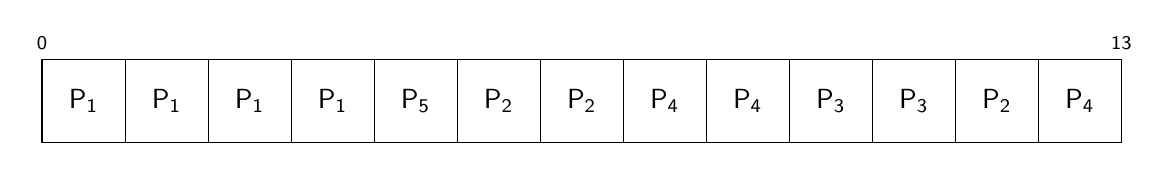
\begin{tikzpicture}

    \draw (0,0) rectangle (39em,3em);

    \foreach \i in {1,...,12} {
      \draw [shorten >=0] (\i * 3em, 0) -- (\i * 3em, 3em);
    }

    \node [anchor=south] at (0em, 3em) {\scriptsize 0};
    \node [anchor=south] at (39em, 3em) {\scriptsize 13};

    \node at ( 1.5em, 1.5em) {$\mathsf{P_1}$};
    \node at ( 4.5em, 1.5em) {$\mathsf{P_1}$};
    \node at ( 7.5em, 1.5em) {$\mathsf{P_1}$};
    \node at (10.5em, 1.5em) {$\mathsf{P_1}$};
    \node at (13.5em, 1.5em) {$\mathsf{P_5}$};
    \node at (16.5em, 1.5em) {$\mathsf{P_2}$};
    \node at (19.5em, 1.5em) {$\mathsf{P_2}$};
    \node at (22.5em, 1.5em) {$\mathsf{P_4}$};
    \node at (25.5em, 1.5em) {$\mathsf{P_4}$};
    \node at (28.5em, 1.5em) {$\mathsf{P_3}$};
    \node at (31.5em, 1.5em) {$\mathsf{P_3}$};
    \node at (34.5em, 1.5em) {$\mathsf{P_2}$};
    \node at (37.5em, 1.5em) {$\mathsf{P_4}$};

  \end{tikzpicture}

  or

  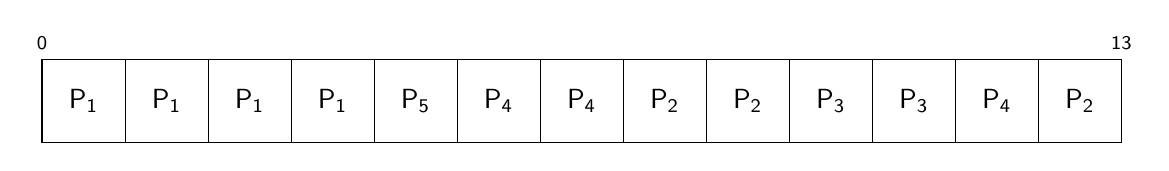
\begin{tikzpicture}

    \draw (0,0) rectangle (39em,3em);

    \foreach \i in {1,...,12} {
      \draw [shorten >=0] (\i * 3em, 0) -- (\i * 3em, 3em);
    }

    \node [anchor=south] at (0em, 3em) {\scriptsize 0};
    \node [anchor=south] at (39em, 3em) {\scriptsize 13};

    \node at ( 1.5em, 1.5em) {$\mathsf{P_1}$};
    \node at ( 4.5em, 1.5em) {$\mathsf{P_1}$};
    \node at ( 7.5em, 1.5em) {$\mathsf{P_1}$};
    \node at (10.5em, 1.5em) {$\mathsf{P_1}$};
    \node at (13.5em, 1.5em) {$\mathsf{P_5}$};
    \node at (16.5em, 1.5em) {$\mathsf{P_4}$};
    \node at (19.5em, 1.5em) {$\mathsf{P_4}$};
    \node at (22.5em, 1.5em) {$\mathsf{P_2}$};
    \node at (25.5em, 1.5em) {$\mathsf{P_2}$};
    \node at (28.5em, 1.5em) {$\mathsf{P_3}$};
    \node at (31.5em, 1.5em) {$\mathsf{P_3}$};
    \node at (34.5em, 1.5em) {$\mathsf{P_4}$};
    \node at (37.5em, 1.5em) {$\mathsf{P_2}$};

  \end{tikzpicture}
  \end{center}
}{
  \vspace{6em}
  \begin{center}
  \begin{tikzpicture}

    \draw (0,0) rectangle (39em,3em);

    \foreach \i in {1,...,12} {
      \draw [shorten >=0] (\i * 3em, 0) -- (\i * 3em, 3em);
    }

    \node [anchor=south] at (0em, 3em) {\scriptsize 0};
    \node [anchor=south] at (39em, 3em) {\scriptsize 13};
  \end{tikzpicture}
  \end{center}
  \vspace{6em}
}

\vspace{1em}

\textbf{(3 points)} What's the average response time?
(Your answer can be fractional.)

\vspace{1em}

\ifbool{solutions}{
  \begin{center}
  $\mathsf{Avg_{ResponseTime} = \frac{0 + 0 + 2+ 6 + 1}{5} = \frac{9}{5} = 1.8}$

  \vspace{0.5em}

  or

  \vspace{0.5em}

  $\mathsf{Avg_{ResponseTime} = \frac{0 + 2 + 2+ 4 + 1}{5} = \frac{9}{5} = 1.8}$
  \end{center}
}{
  \vspace{8em}
}

\textbf{(4 points)} What's the average waiting time?
(Your answer can be fractional.)

\ifbool{solutions}{
  \begin{center}
  $\mathsf{Avg_{WaitingTime} = \frac{0 + 4 + 2 + 9 + 1}{5} = \frac{16}{5} = 3.2}$

  \vspace{0.5em}

  or

  \vspace{0.5em}

  $\mathsf{Avg_{WaitingTime} = \frac{0 + 5 + 2 + 8 + 1}{5} = \frac{16}{5} = 3.2}$
  \end{center}
}{
}

\newpage

\textbf{(10 points total) Page Tables.}

\vspace{1em}

Your system has 2 MiB ($\mathsf{2^{21}}$) pages, a PTE size of 8 bytes, and
uses 57 bit virtual addresses. You decide to use multi-level page tables, and
fit each smaller page table on a single page.

\vspace{1em}

\textbf{(2 points)} How many PTEs can you fit into a single smaller page
table? (Answer can be a power of 2.)

\vspace{1em}

\ifbool{solutions}{
  \begin{answer}
    You could fit $\mathsf{2^{18}}$ PTEs into a page size of 2 MiB.
  \end{answer}
  \vspace{3em}
}{
  \vspace{4em}
}

\textbf{(4 points)} How many levels do you need for your multi-level page table?
Show your work.

\vspace{1em}

\ifbool{solutions}{
  \begin{answer}
    You need 2 levels for your multi-level page table.

    $\mathsf{\lceil \frac{57 - 21}{18} \rceil = \lceil \frac{36}{18} \rceil
      = 2}$
  \end{answer}
  \vspace{4em}
}{
  \vspace{10em}
}

Now that you have a multi-level page table with \textit{n} levels (if you
didn't calculate \textit{n} you can assume a value greater than 1).
You want to calculate the effective access time of this approach.
On this system it takes 10 ns to search the TLB, each memory access takes 100
ns, and we have a hit rate of 50\%.
Recall that for a single page table the equation for effective access time is:

\begin{center}
$\mathsf{EAT = \alpha \times TLB_{HitTime}
               + (1 - \alpha) \times TLB_{MissTime}}$
\end{center} \vspace{-2em}
\begin{align*}
  \mathsf{where} \\
  \mathsf{TLB_{HitTime}} &= \mathsf{TLB_{Search} + Mem} \\
  \mathsf{TLB_{MissTime}} &= \mathsf{TLB_{Search} + 2 \times Mem}
\end{align*}

\textbf{(4 points)} Calculate the effective access time for this multi-level
page table. Show your
work.

\ifbool{solutions}{
  \vspace{1em}
  \begin{answer}
    You need 2 levels for your multi-level page table. Therefore on a TLB
    miss you need 3 memory accesses, one for each level of the page table and
    one for the original access.

    \begin{align*}
      \mathsf{TLB_{HitTime}} &= \mathsf{10\ ns + 100\ ns} \\
      \mathsf{TLB_{MissTime}} &= \mathsf{10\ ns + 3 \times 100\ ns} \\
      \mathsf{EAT} &= \mathsf{0.5 \times 110\ ns + 0.5 \times 310\ ns} \\
                   &= \mathsf{55\ ns + 155\ ns} \\
                   &= \mathsf{210\ ns}
    \end{align*}
  \end{answer}
}{
  \afterpage{\null\newpage}
}


\end{document}
